\documentclass[11pt]{extarticle}

\usepackage{tikz}
\usepackage{titlesec}
\usepackage[top = 3cm]{geometry}

\newcommand{\sectionbreak}{\clearpage}

\usepackage[hypertexnames=false]{hyperref}

\hypersetup{
    colorlinks,
    citecolor=black,
    filecolor=black,
    linkcolor=black,
    urlcolor=black,
    linktoc=all
}

% \renewcommand{\thesection}{\Alph{section}}
\renewcommand{\theHsection}{\Alph{section}}

\title{\Huge{Documentation for the dungeon project}}
\author{Quentin GUEZ}
\date{}

\begin{document}

\maketitle

\tableofcontents

\clearpage

\part{Game description}

\section{Explanation of the game}

You are controlling Thorn, a young adventurer and you have a new quest in this adventure. You're trying to gather all the four Statues of Youth. They will let you make any wish you want. Unfortunately, those statues are being kept by the terrible Girk. He's been keeping them for years as his glorious treasure. Now has come the time for you to pick them up and make any wish come true.

On your way to the statues, you will face many dangers. You'll start outside where there's only one door facing you. You will therefore have to make choices about where you choose to go. 

If you meet an enemy, you will have a two options : try to flee but with a low chance of success, or directly attack and bravely face the danger. But be careful, you don't know how strong the enemy is yet. 

If you get lucky on your way, you might find a magic key that can unlock any door. But be aware that you can only use one per door. You can also find weapons or potions on your way so watch your steps.

\section{List of the functionnalities}

\begin{itemize}
    \item move between rooms
    \item play music
    \item describe each room's name
    \item check the player's stats
    \item fight an enemy 
    \item choose an attack
    \item double attack with random chance of success
    \item possibility to flee and escape the enemy as long as you don't go back to the room
    \item music and a description for each transition
    \item rooms can be locked or opened
    \item possibility to find items (key, potion, statue)
    \item different weapons are available
    \item a player can steal the enemy's weapon once he has beaten him
    \item a player can take any weapon he finds
    \item a menu is displayed at the start
    \item the user can choose whether he wants to unlock the door with a key or not
\end{itemize}

\clearpage

\part{Code documentation}

\setcounter{section}{0}

\section{The folders tree / the architecture}

\begin{figure}[ht]
    \centering
    
    \caption{the architecture of the application}
    \label{architecture}
    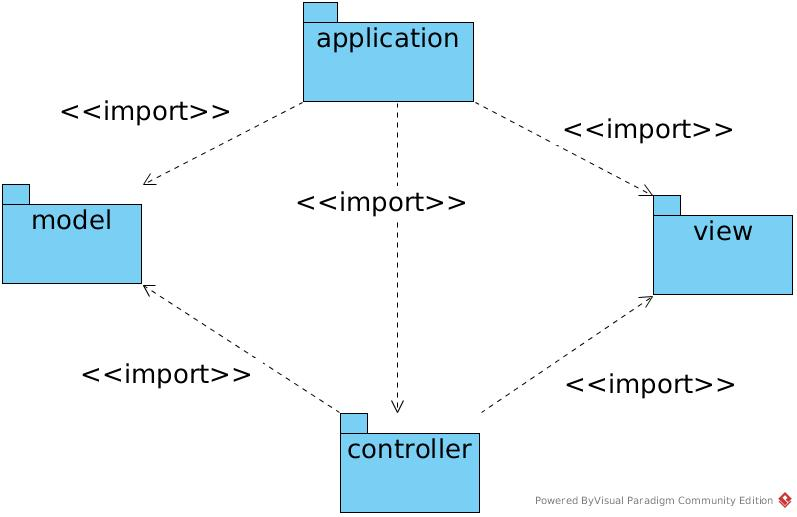
\includegraphics[scale = 0.4]{architecture}
\end{figure}

This project is separated in several packages. This is following the MVC (Model, View, Controller) pattern. 

Firstly, there's the view packages. All of the text printed is from this package. There's two classes in this package : DungeonView and MenuView. Their name speaks for themselves. The MenuView class displays all the text of the Menu and the other one, displays all the text for the game.

Then, the model package. This is the biggest one. It contains the classes and enumerations of all the elements used in the project. There's a lot of them so I'm not going to list them.

To complete our MVC, the controller package includes the model and the view packages to basically control them. It checks the state of the model to display the corresponding text from the view package.

Eventually, there's the application which only contains one class called Main. This class is the one executed to run the project. It's really simple and just calls the MenuController to start.

You can see it represented on figure \ref{architecture}.

\section{The scenario}

\begin{figure}[hb]
    \centering
    
    \caption{the menu}
    \label{menu}
    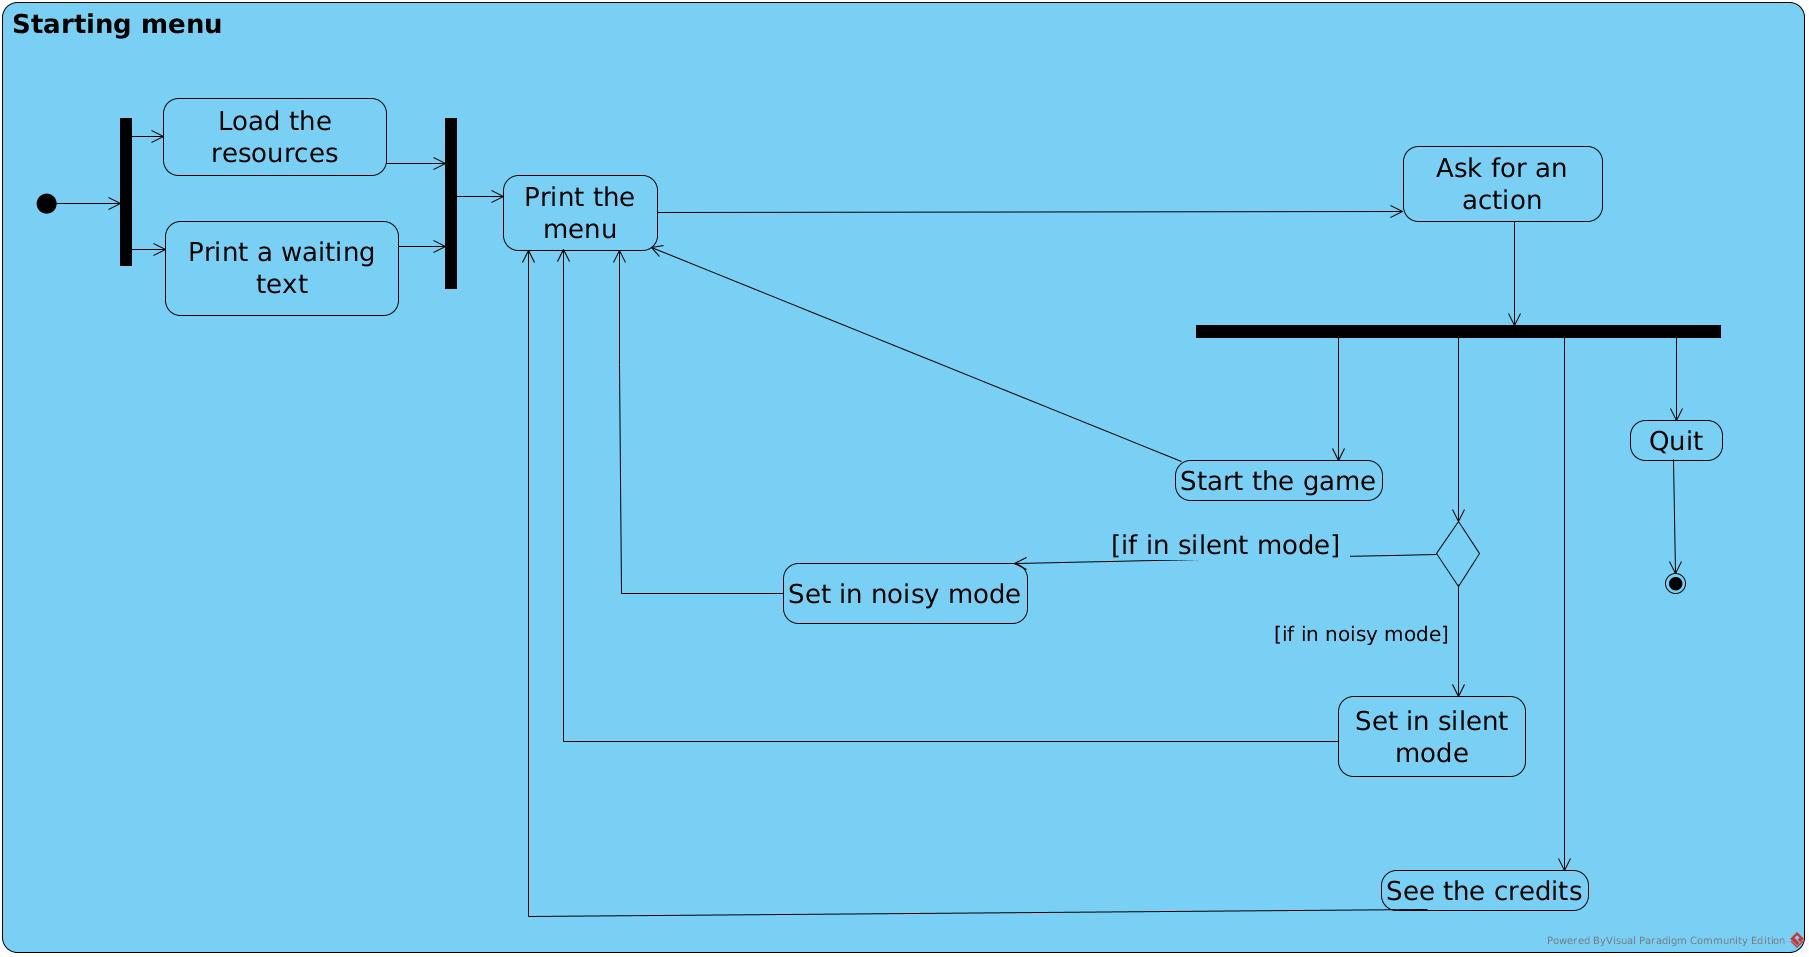
\includegraphics[scale = 0.198]{menu}
\end{figure}

When you run the application, you first have to wait until all the resources are loaded. Don't worry, you won't have to wait long everytime ! It detects whether the resources are already present on the computer. 

Once the resources are ready, the menu is displayed. It has four options and lets the user choose among them. After each choice, the menu is displayed again.

If the player has the game set with no sound it would suggest to play it with sound and vice versa.

Once the player is satisfied, the player can start the game.

If needed, the player can check the credits.

The user has also the posibility to quit through this menu. 

All of this is detailed in figure \ref{menu}.

\begin{figure}
    \centering
    
    \caption{the game}
    \label{game}
    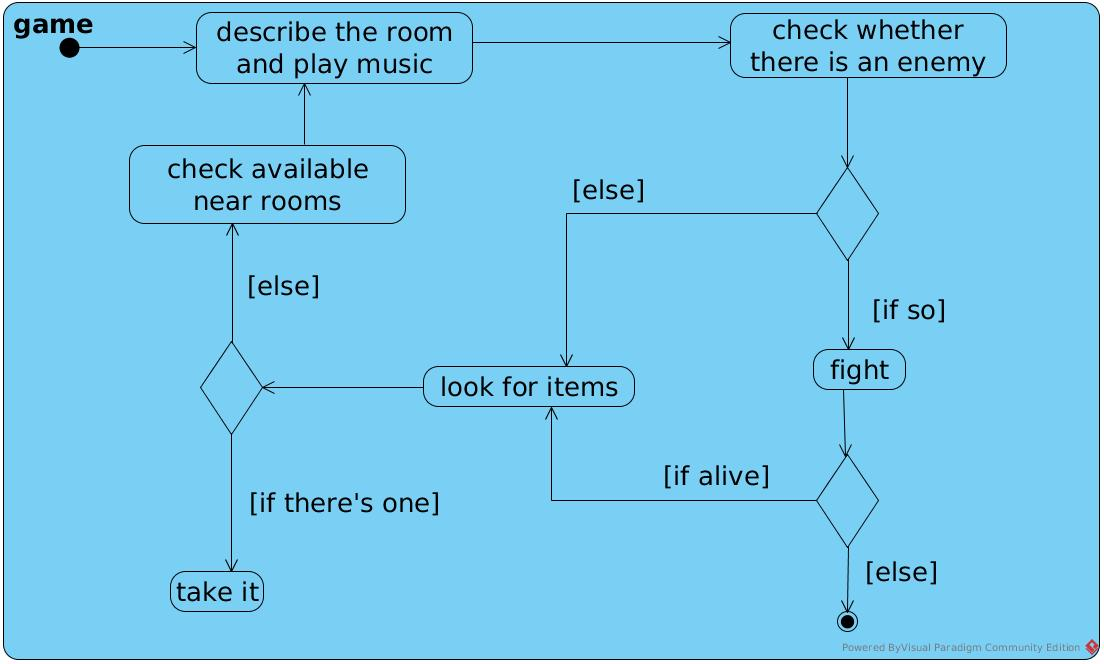
\includegraphics[scale = 0.32]{game}
\end{figure}

\vspace{\baselineskip}

Once the game is started, it continuously executes the following actions. It starts by describing the current room of the player and playing the music associated to the room. It then checks for the presence of an enemy in the room. If there's one, then there is a fight otherwise it just looks for items. If the player dies during the fight, the game is over. But if not, then we can go back to looking for items. It continuously looks for one until there's none of them left. Once it's done, it checks the available rooms to go and restart it. You can see that in the figure \ref{game}.

\section{The loading of the resources}

\begin{figure}[ht]
    \centering
    
    \caption{the loading of the resources}
    \label{resources}
    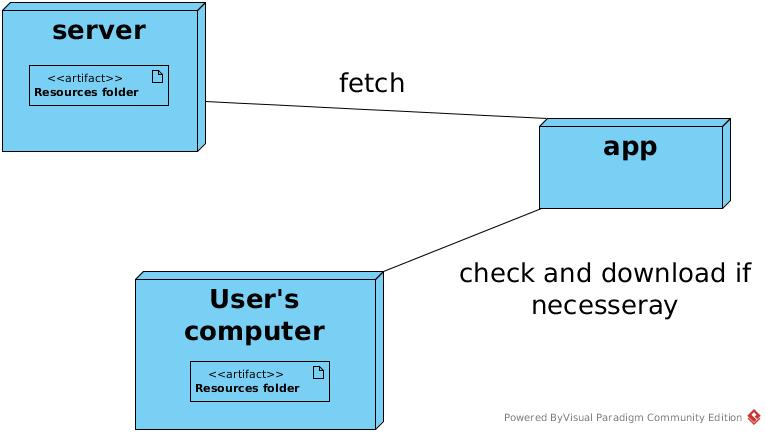
\includegraphics[scale = 0.46]{resources}
\end{figure}

All the resources for the game (which actually only contains the sounds) are stored on a server. The program fetches those data and recreates the corresponding folders present on the server to the user's computer. It also checks whether it already exists. 

This is shown in figure \ref{resources}.

\section{The main classes}

\begin{figure}[b]
    \centering
    
    \caption{the Dungeon class}
    \label{dungeonClass}
    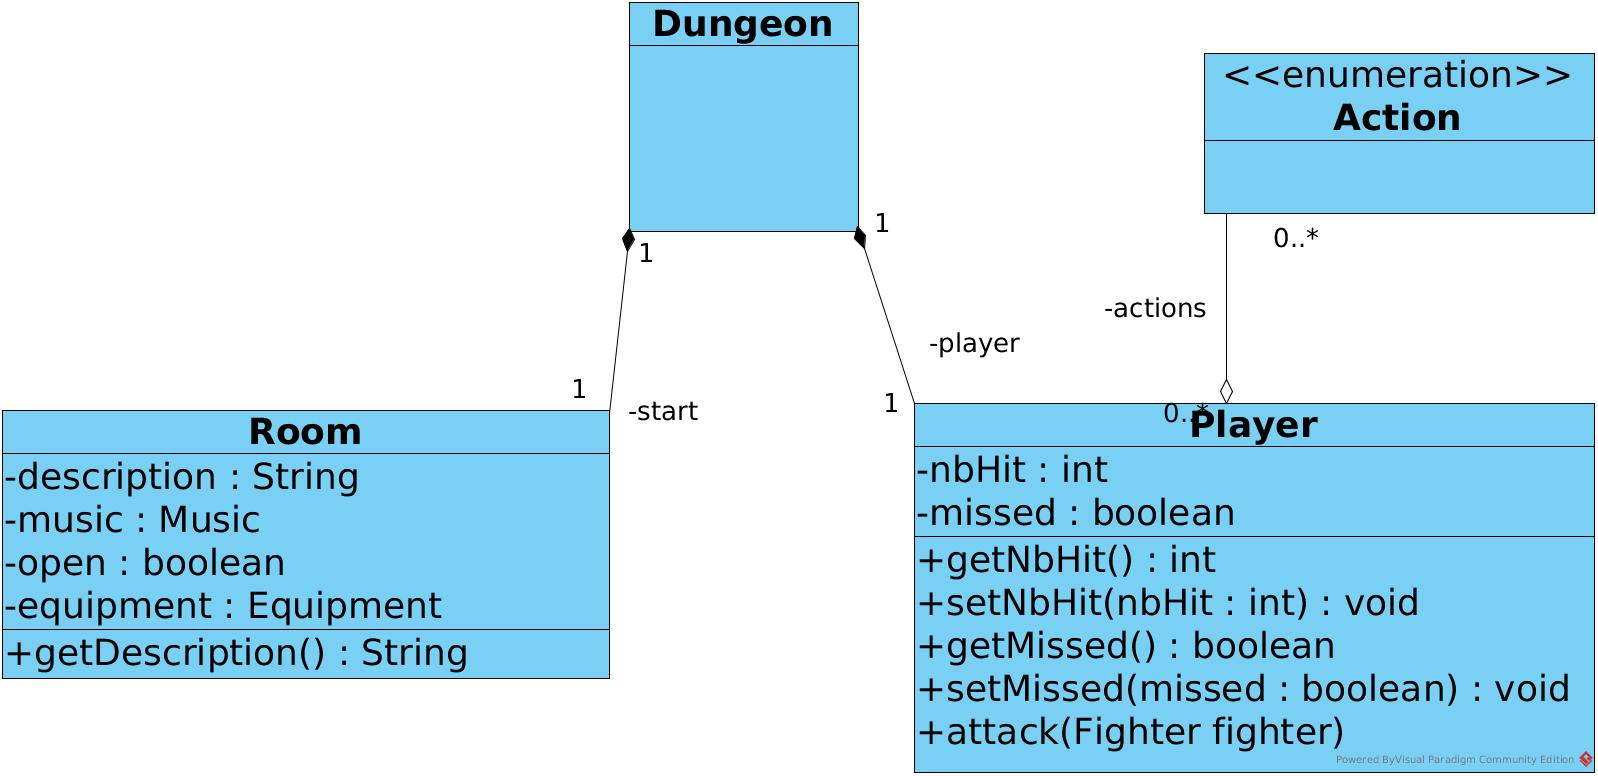
\includegraphics[scale = 0.2]{dungeon}
\end{figure}

\begin{figure}
    \caption{the Room class}
    \label{roomClass}
    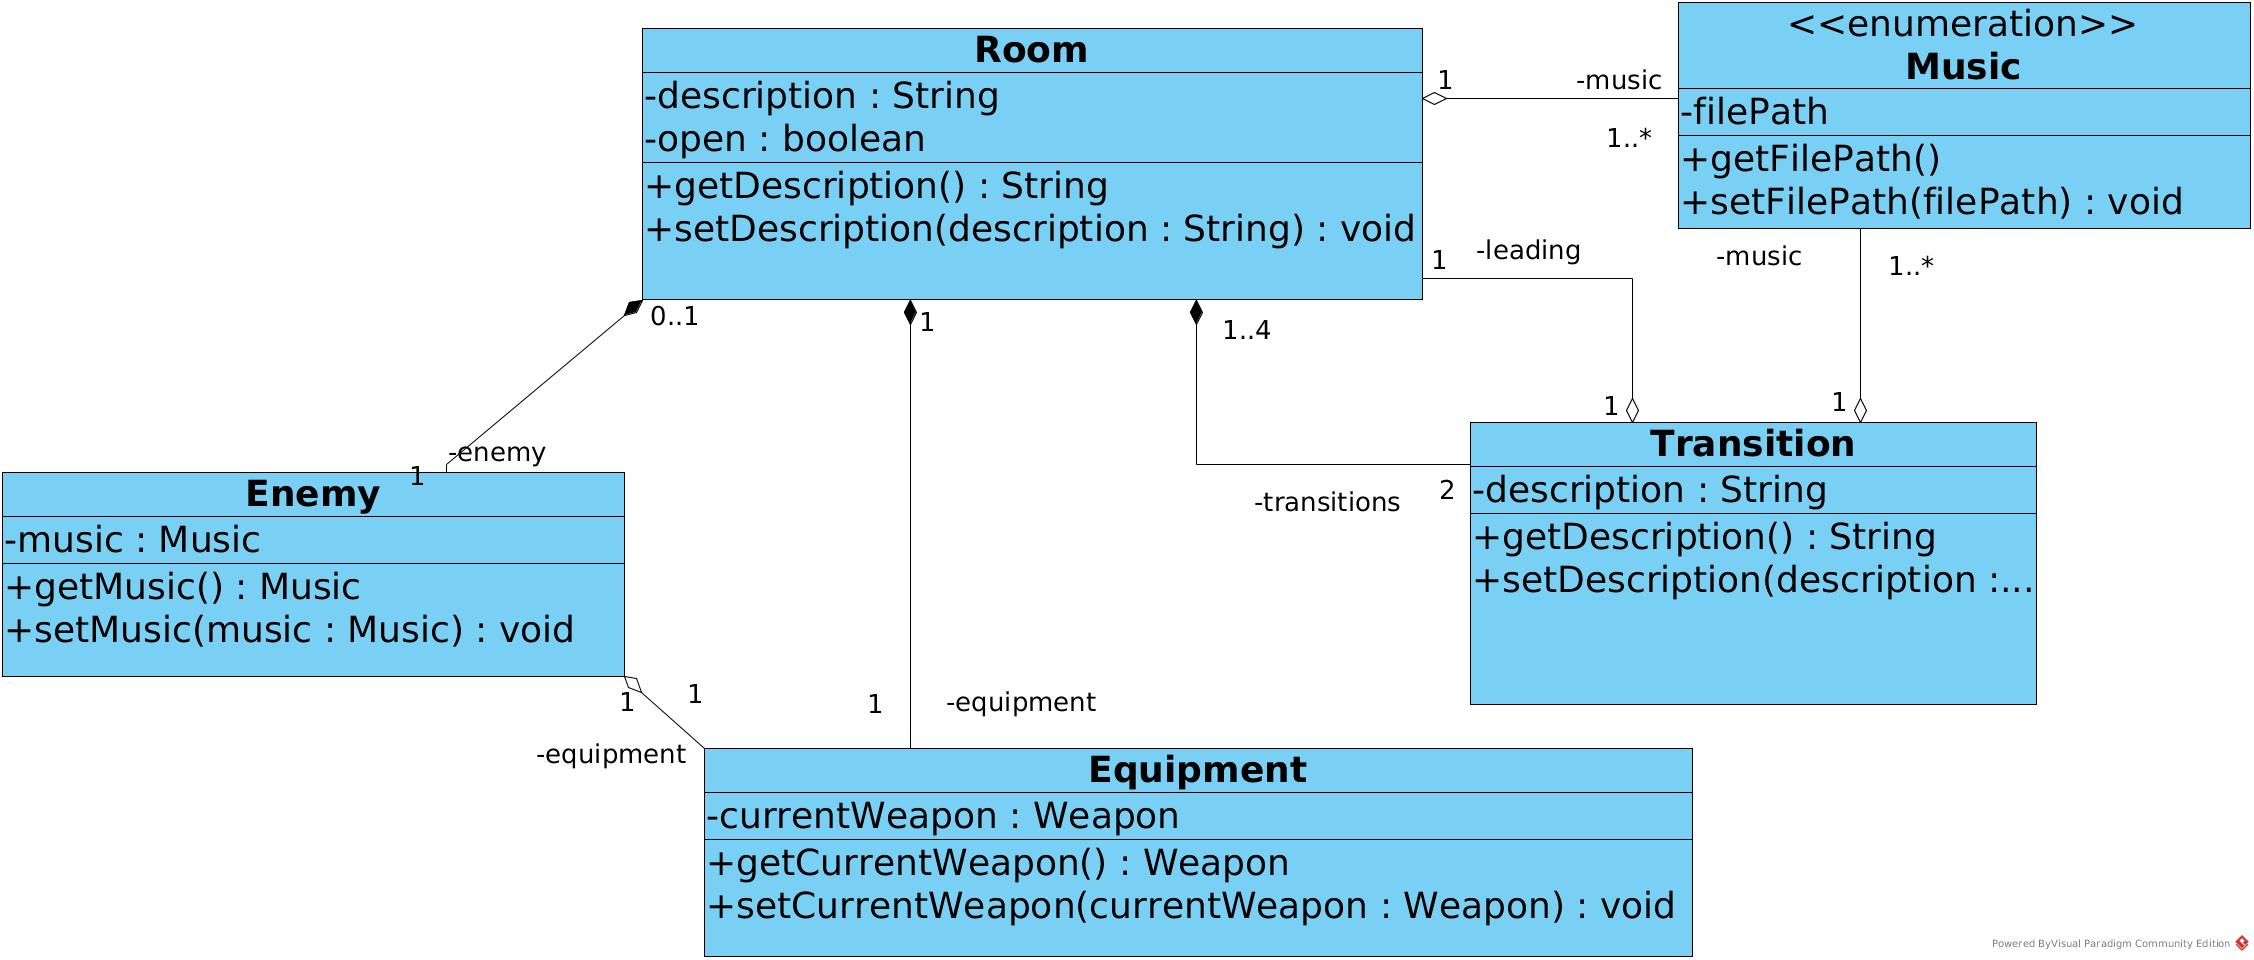
\includegraphics[scale = 0.15]{room}
\end{figure}

\begin{figure}
    \centering
    
    \caption{the Character class}
    \label{characterClass}
    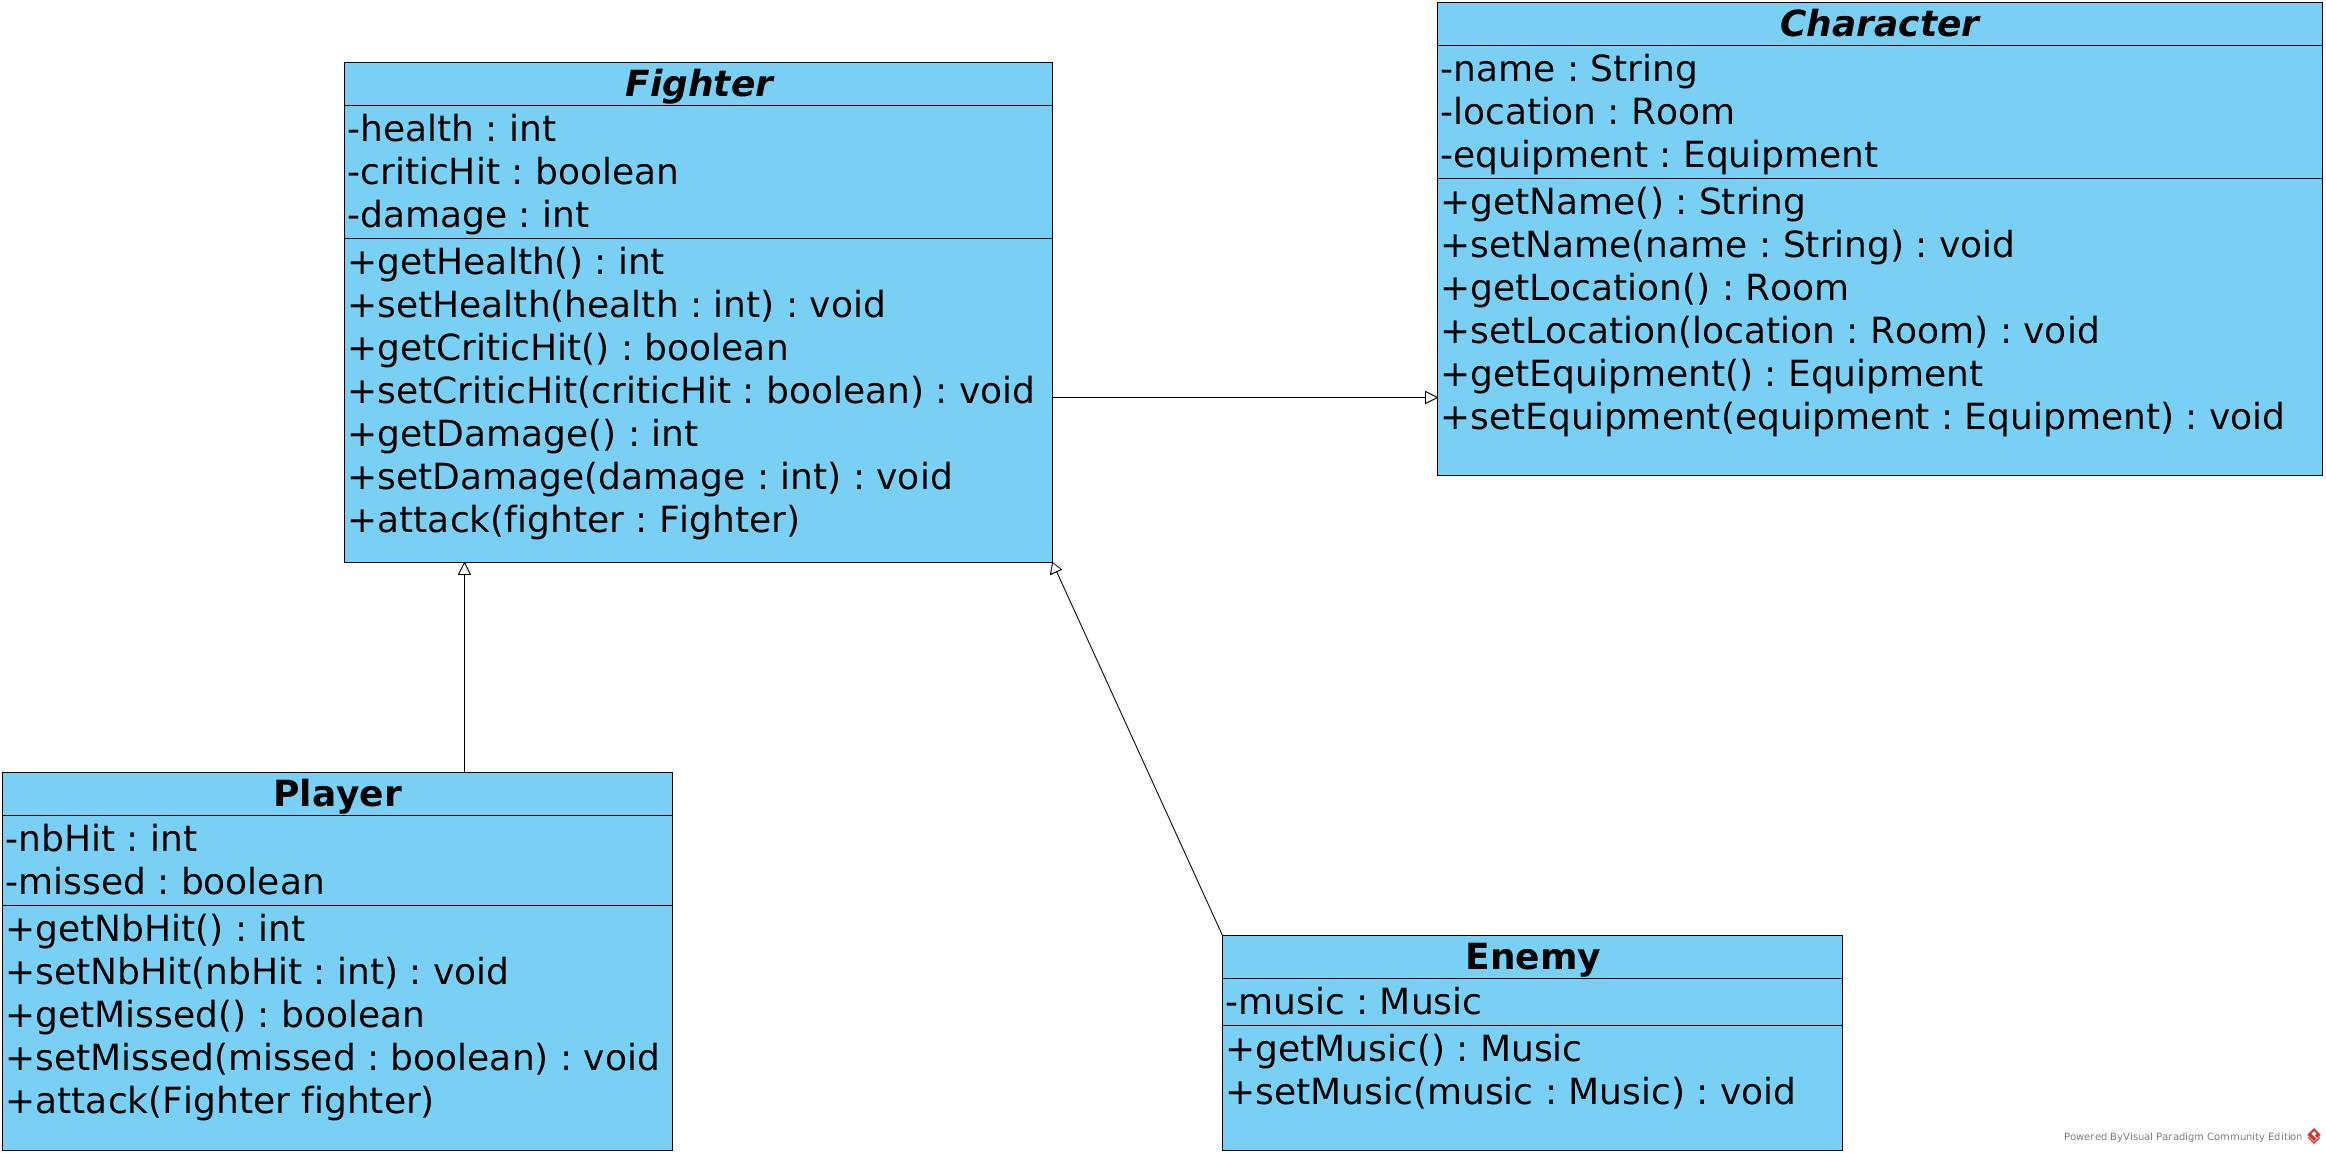
\includegraphics[scale = 0.15]{character}
\end{figure}

\begin{figure}
    \centering
    
    \caption{the equipment}
    \label{equipmentClass}
    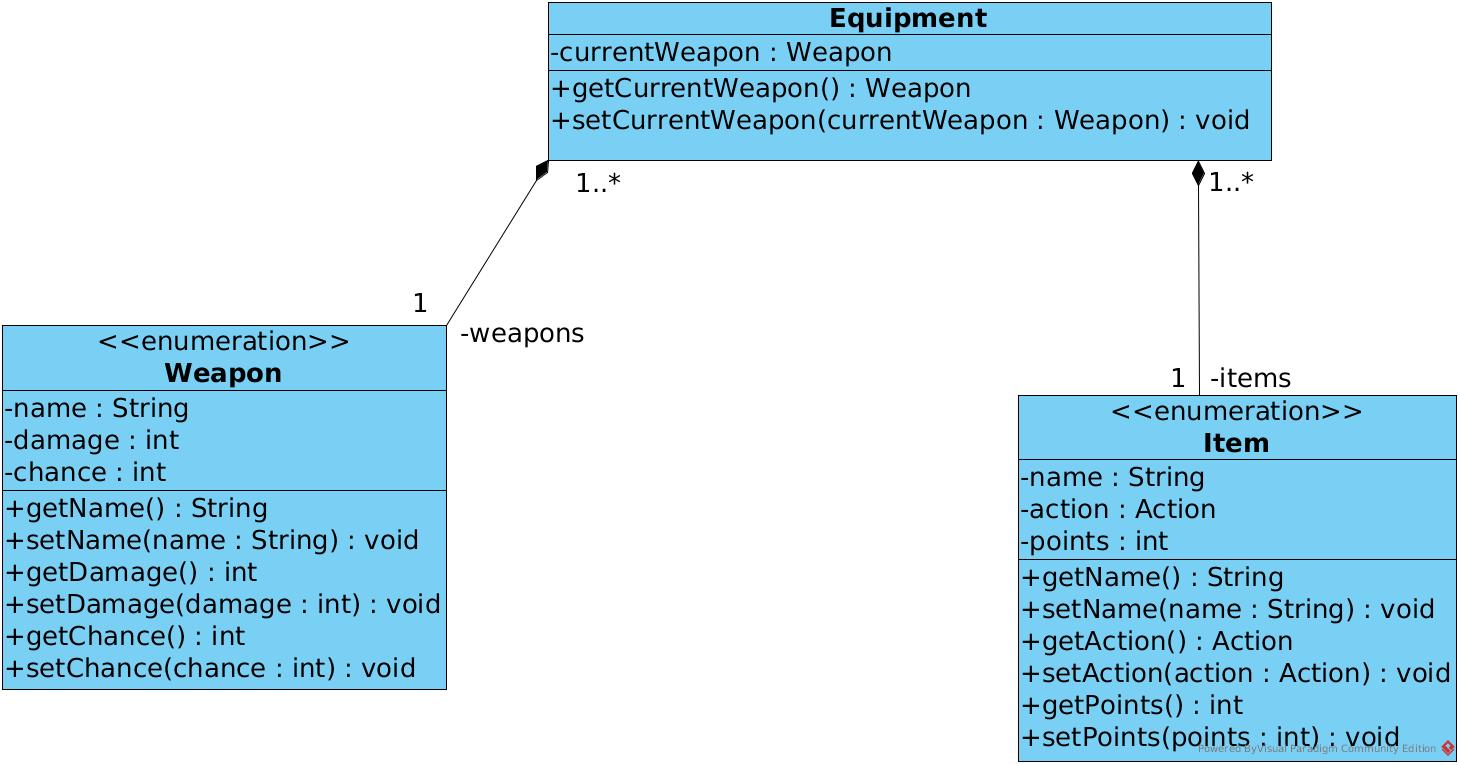
\includegraphics[scale = 0.24]{equipment}
\end{figure}

The class dungeon is the main class of the project. But it doesn't contain a lot of classes. It only needs to keep the starting room and the player. All the other rooms will be linked to each other. The dungeon doesn't have any particular method, all of them are in the controller.

The Room class is composed of a description, music, a boolean whether it is opened and equipment. 

The Player class is composed of a nbHit variable that counts the number of standard attacks he's done, and a missed boolean variable that stores whether he missed his powerfull attack or not. It also holds all the actions available for the player, within a list of Action enumeration.

You can see all of that on the class diagram in figure \ref{dungeonClass}

\vspace{\baselineskip}

The Room class has a link to another room through the Transition class. It can have an enemy and is composed of equipment and music. 

The Transition class has a description, music and a room that it leads to.

An Enemy has equipment and music.

Music is an enumeration that has a filePath.

You can the diagram represented on figure \ref{roomClass}

\vspace{\baselineskip}

The Character class specifies the structure of a character. This class is abstract. It has a name of type String, a location of type Room and and an equipment of type Equipment. 

The Fighter class is also abstract and inherits from Character. It defines what a fighting character would do and therefore has health and damage attributs. It also contains a boolean whether he's making a criticHit.

We then have the Player class which extends the Fighter class. It adds a nbHit variable that hold the number of standard hits he's made (not critic ones) and a missed boolean. It redefines the attack method because a player attack is different.

Finally, we have an Enemy class which also extends the Fighter but adds a Music to it.

You can see all the classes represented in figure \ref{characterClass}.

\vspace{\baselineskip}

The equipment class is composed of two enumerations Item and Weapon. In addition, it contains a current weapon. 

A weapon has a name, a damage value and a chance of success for a critic attack. 

An item has a name and an action, plus an optional attribute which is the points to earn (for the potion item). You can see it in details on figure \ref{equipmentClass}.

\section{The player's movement}

\begin{figure}[hb]
    \centering
    
    \caption{the player movement}
    \label{playerMovement}
    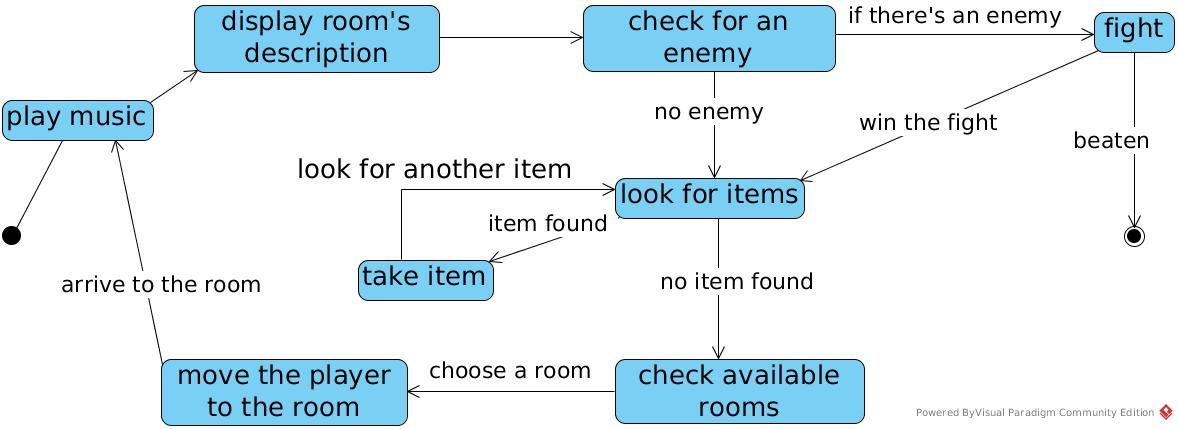
\includegraphics[scale = 0.3]{player's movement}
\end{figure}

Here's what happens when a player moves. The controller plays the music of the current room. It then calls the view to display the description of that room before checking for any enemy in the room. 

If it finds an enemy, then a fight starts between the player and the enemy. If the player loses, the game ends. Otherwise, the controller looks for an item. If there's one found, the view prints it and the user is asked to take it. Then it goes back to looking for item. 

Once there's no items left, it checks the available rooms and then asks the user to choose one and move the player in consequence. It then goes back to the first step and it starts again. The corresponding state diagram is on figure \ref{playerMovement}.

\section{The player's actions}

\begin{figure}[h]
    \centering
    
    \caption{the player's actions}
    \label{playersActions}
    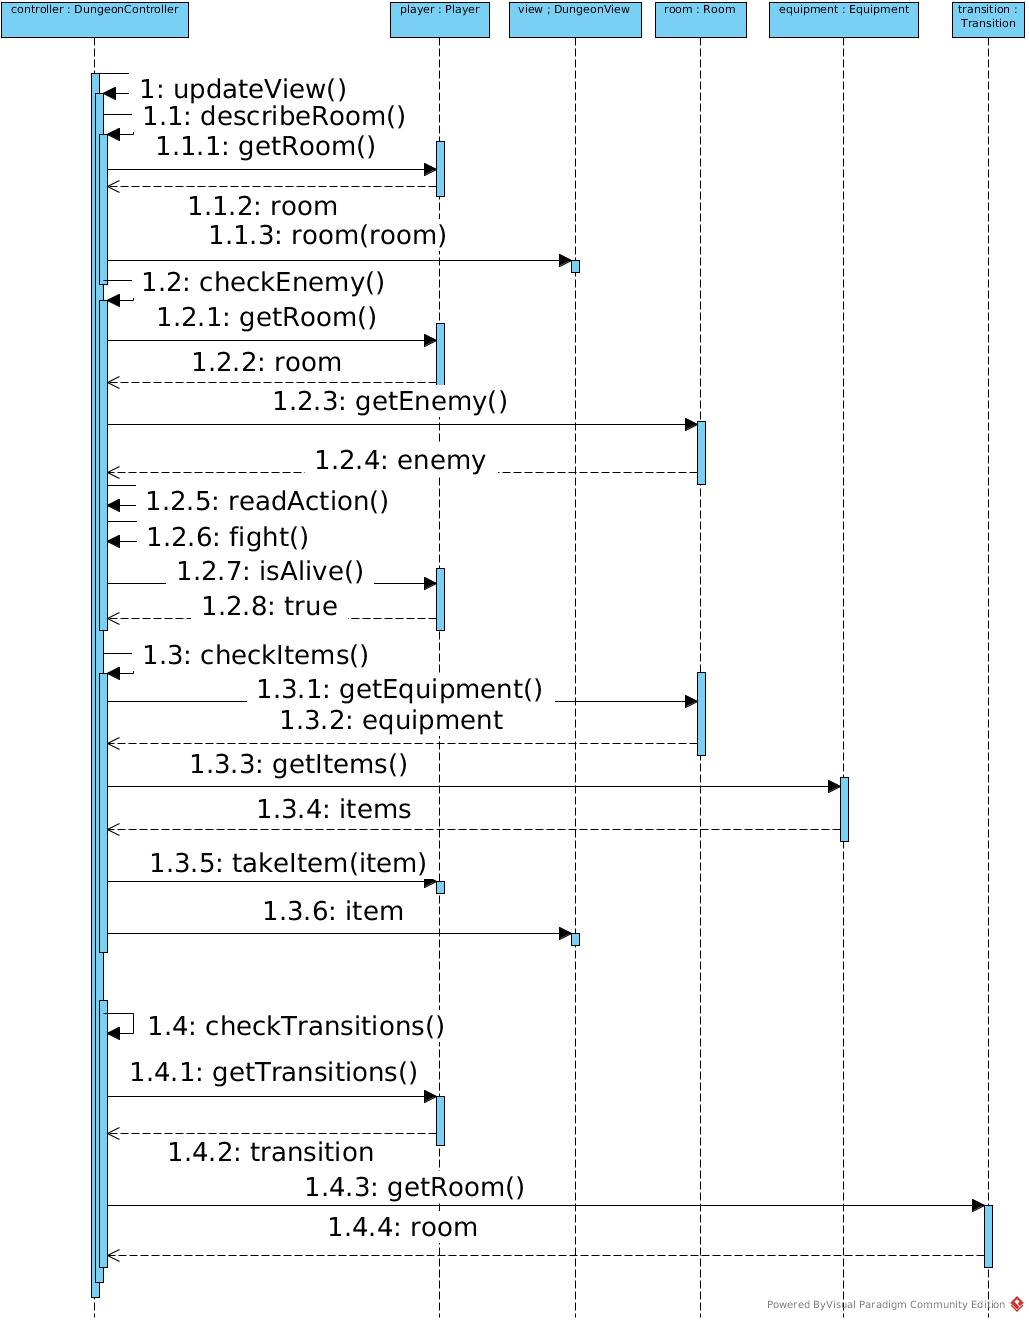
\includegraphics[scale = 0.34]{player's actions}
\end{figure}

The DungeonController class has a recursive method called updateView. It is called again and again until the player is dead. 

The thing this function does is it describes the current room, which the room of the player. To do so, it asks the player class to return the room and then plays the music associated and calls the view to display its description.

After describing the room, it checks the presence of an enemy in the room. The method checkEnemy starts by getting the room of the player. If this room doesn't contain an enemy, it quits. Otherwise, a fight starts. If the player doesn't come out alive, the game ends and the function updateView quits. 

Afterwards, the items in the room are being checked. The controller calls the equipment's getter of the class room to check it. It then prints it with the view class before checking again until there's none left. 

Finally, the checkTransitions method is called. This method loops through all the rooms next to the current one. The method updateView can start over again.

All of this is summarized in a sequence diagram on figure \ref{playersActions}.

\section{The fight}

When a fight starts, the user is asked for executing actions. Two actions are added : flee or attack. If the user tries to flee, it calls the static method of the class Console to generate a 10\% chance of success and quits in case of success.

Else, the user is asked to choose their weapon. 

Once the weapon is chosen, the fight method is called. 

The fight method is recursive. It starts by asking for a type of attack, either a standard one or a powerfull one which has a chance of success limited but does twice of damages as a standard one. A standard hit increases the chance of succes of a powerfull one. 

Once it has the type of attack, it calls the method attack from player. Prints the actions with the view and recall this function with a different boolean for the enemy turn. 

When the player defeats their enemy, the defeat method from the view object is called. The room's equipment is called to steal the enemy's equipment with the method steal of the class Equipment.

A summary of those actions is available on figure \ref{fight}.

\begin{figure}[th]
    \centering
    
    \caption{a fight}
    \label{fight}
    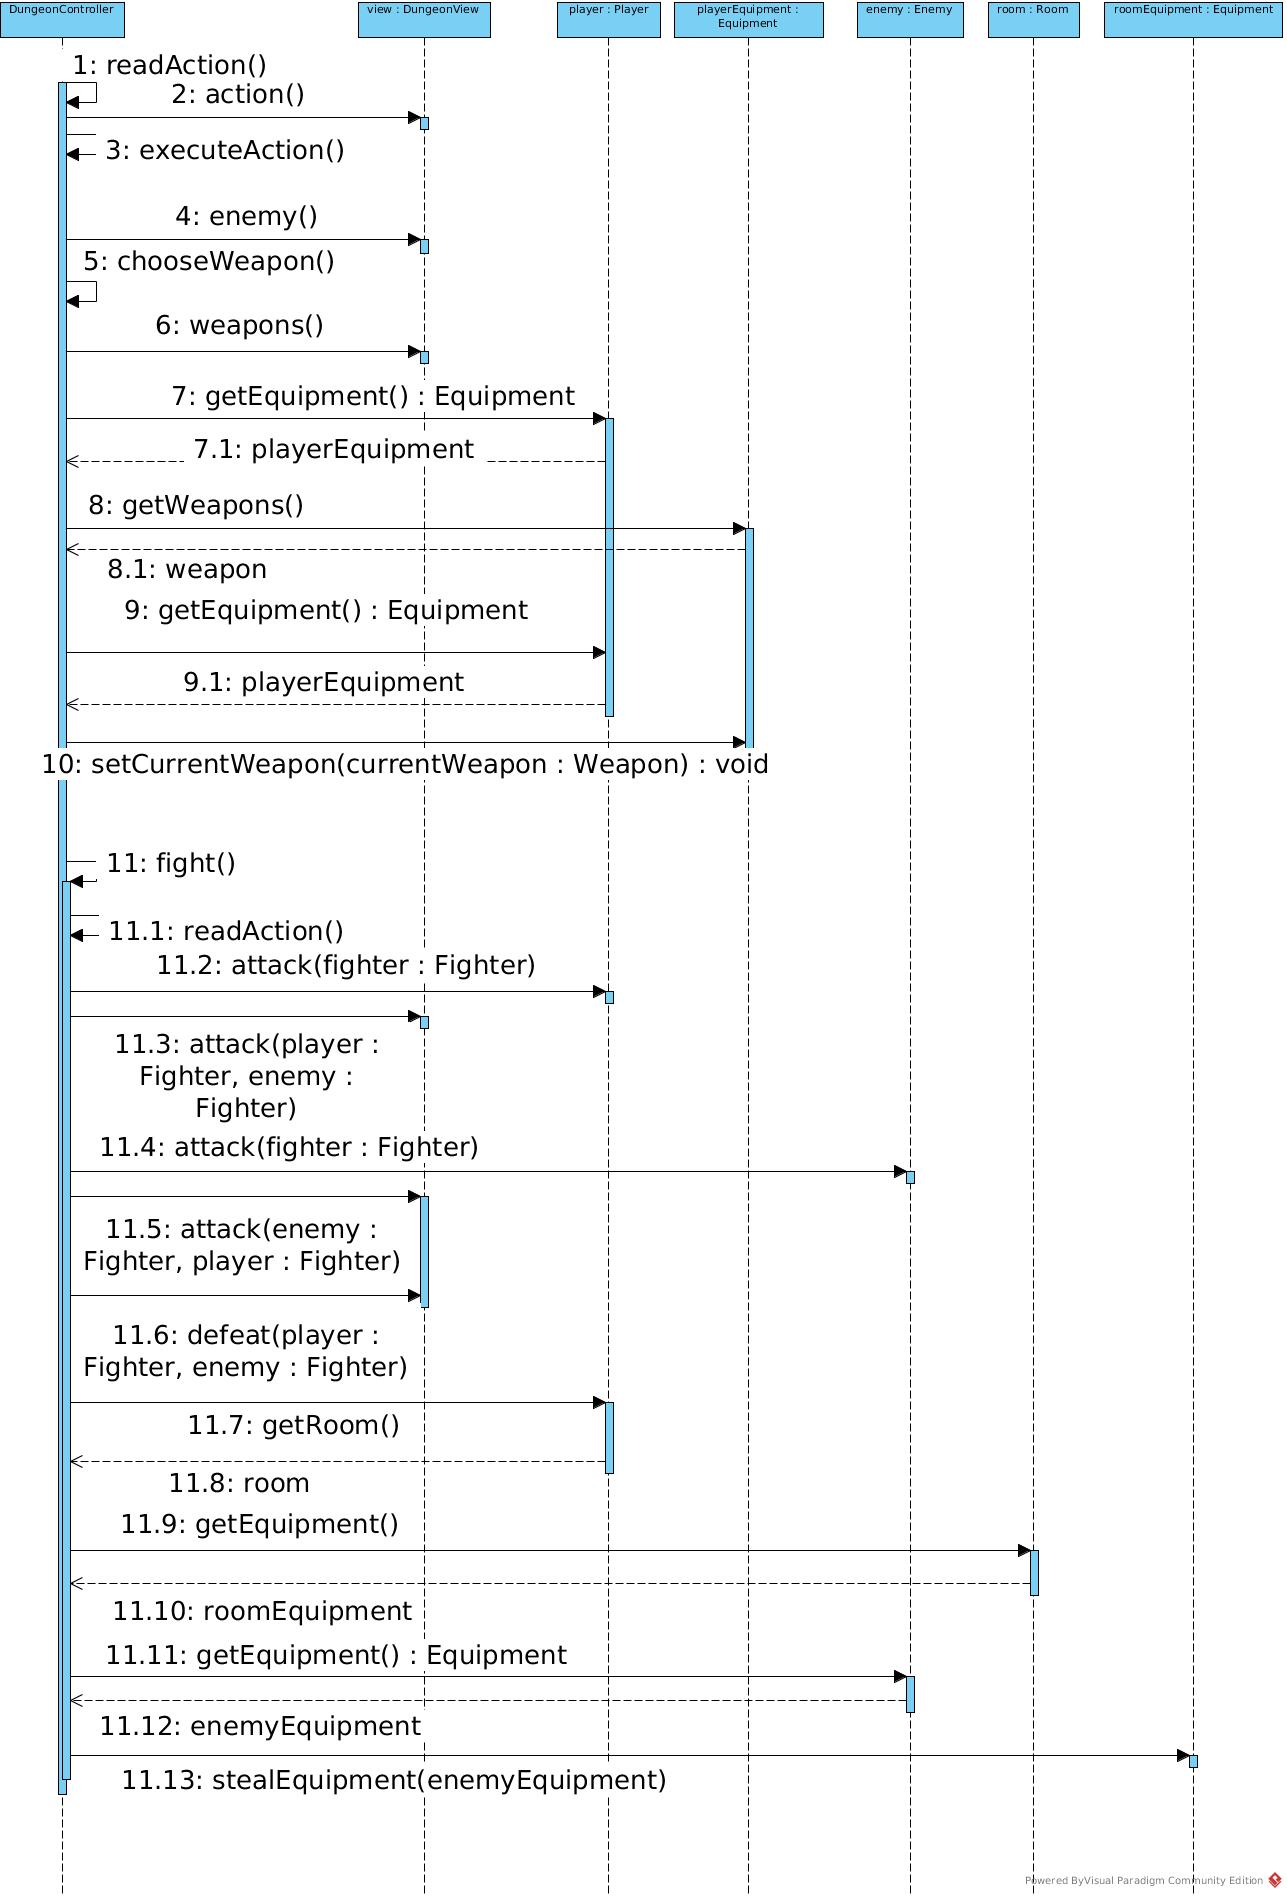
\includegraphics[scale = 0.25]{fight}
\end{figure}

\part{Conclusion}

\setcounter{section}{0}

\section{Bonus}

I originally planned to do more and this is what I'm going to talk about in this section. When I started the project, I asked my brother if he had an idea of a good scenario for a level. He actually proposed that the game would start with a room where you face a door and you have to choose between knocking or breaking the door which would lead to different path. I haven't found a way to modelise this, so I eventually gave up on this idea.

I also wanted to include some XML in the project. To do so, I had this idea of letting the opportunity to the user to create their own game. To do that, I firstly needed to be able to store the level I created in an XML file which failed. This is when I gave up on this idea and stopped coding this project for days. But I had already planned how to manage that.

I would send on the server the newly created levels in the form of an XML and so whenever someone would play the game, the newly created levels would be downloaded. Everybody would then be able to access the levels that anyone would have created. They would simply need to select it from the menu. 

To create a level in an easy way, the user would be asked to create each room first until they are done. They would be asked to add any of the possible elements you can add in a room. Once they finished adding the elements into the room, they would have to provide a name. All of this would be added and stored in a room object. And all the rooms would be stored in a dictionnary (HashMap in java) which gives a room for a given String (the name of the room chosen by the user). Once all of the rooms are completed, they will have to link them. The program would make sure that the level is well linked (which I haven't figured out yet). Finally, this would create a Game object. This object would be mapped into an XML file and sent to the server.

But unfortunately, none of that has been done because I haven't planned at the start about making my Dungeon able to be mapped into an XML file. 

\section{My mistakes}

When I was coding, I realized that there were some mistakes that I made. 

To start, as you might realize from seeing my project, I've been way too ambicious compared to the required work and my capacities as well. But this was also a good challenge for me, which is why I like to be ambicious and curious. I've learnt a lot throughout this project and especially from my mistakes. I relieved the following mistakes.
 
I started too fast. As I said, I asked to my brother for an idea of a scenario and I directly wanted to do exactly like he said. That's wrong. I should start by doing some basic elements, and then add the more complex ones. This also links to the idea of mapping my Dungeon into an XML file. If I had thought about it earlier, I would have probably done it. 

Another important mistake was the lack of test. Actually, I did none. Next time, I will test every part of my program using the JUnit class. 

To be more organised, I should use UML more often. I only did one diagram before coding. And it wasn't the best diagram. It was huge and unreadable. 

Finally, starting the documentation in the last week, the last days was a bad idea. I have to come back to what I was thinking the moment I did it\dots That's wrong. I should write the documentation every time I finished and verified a part of my program. This would help me later.

Though, I can also note the good thing I did for this project. I used my pen and my paper a lot which helped me in many situations. And I also used git pretty well which happened to be pretty useful in some situations.

\end{document}